\clearpage
\begin{examplebox}

	\textbf{\textcolor{CExample}{例1（基础）}}

	\textbf{\textcolor{CExample}{题目：}}
	设$f_a(x)=\log_a(x-1)$（$a>0$且$a\ne1$），求定义域，并找出对所有合规底数$a$都不变的图像定点。

	\textbf{为什么想到：}真数大于0决定定义域，真数等于1决定定点。

\begin{center}\begin{tikzpicture}[font=\small,>=stealth,line join=round]
\draw[gray!40,rounded corners=3pt] (0,0) rectangle (14.2,6.2);\node at (7.1,5.6000000000000005) {例1：先保留x大于1，再令真数等于1找定点};
\node[anchor=west] at (.8,4.55){$x-1>0\ \Longleftrightarrow\ x>1$};\draw[->,gray] (2,4)--(12.7,4);\draw[blue!75!black,very thick,->] (5.5,4)--(12.25,4);\draw[blue!75!black,fill=white] (5.5,4) circle(2.8pt);\node[below=6pt] at (5.5,4){$1$};\node[anchor=west] at (.8,2.7){令真数$x-1=1$};\draw[->,gray] (2,2.15)--(12.7,2.15);\fill[orange!85!black] (7,2.15) circle(2.8pt);\node[below=6pt] at (7,2.15){定点横坐标$2$};
\node[text width=12.6cm,align=center] at (7.1,.65) {定义域端点1不取；真数为1时x=2，得到共同点(2,0)。};
\end{tikzpicture}\end{center}

\textbf{\textcolor{CExample}{解题步骤：}}
	\begin{description}[style=nextline, leftmargin=2.8em, labelsep=0.5em, itemsep=0.45em]
		\item[\textbf{第一步（求定义域）：}] 由真数$x-1>0$得$x>1$，故定义域为$(1,+\infty)$。
			\par\textbf{理由：} 对数函数要求真数大于$0$。
		\item[\textbf{第二步（找定点）：}] 令$x-1=1$，即$x=2$，此时$f_a(2)=\log_a 1=0$，所以图像恒过定点$(2,0)$。
			\par\textbf{理由：} 当真数为$1$时函数值恒为$0$。
	\end{description}

	\textbf{\textcolor{CExample}{关键结论：}}
	定义域$(1,+\infty)$，\textbf{不随底数改变的}定点$(2,0)$。
\begin{center}
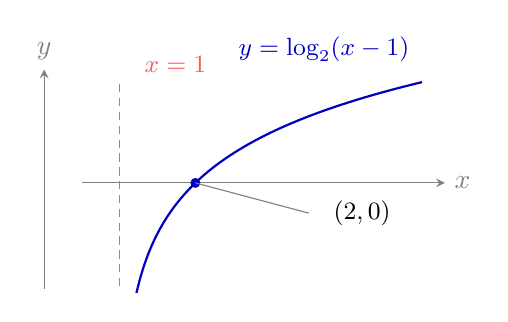
\begin{tikzpicture}[x=0.96cm,y=0.64cm,>=stealth]
  \draw[->,gray] (0.5,0)--(5.3,0) node[right] {$x$};
  \draw[->,gray] (0,-2.1)--(0,2.25) node[above] {$y$};
  \draw[densely dashed,red!65] (1,-2.05)--(1,2.05);
  \draw[thick,blue!75!black,domain=1.22:5.0,samples=75] plot (\x,{ln(\x-1)/ln(2)});
  \fill[blue!75!black] (2,0) circle (1.8pt) ;\draw[gray] (2,0)--(3.5,-.6);\node[anchor=west] at (3.7,-.6){\small $(2,0)$};
  \node[red!65,anchor=west] at (1.2,2.35) {\small $x=1$};
  \node[blue!75!black] at (3.7,2.65) {\small $y=\log_2(x-1)$};
\end{tikzpicture}
\par\small 图仅取$a=2$画出示意；任意合规底数都经过$(2,0)$，$x=1$不能取到。
\end{center}

\textbf{最快判断：}看到$\log_a(\text{式子})$求固定过点，直接令“真数$=1$”；看到定义域，令“真数$>0$”。

	\medskip
	
\end{examplebox}
\clearpage
\begin{examplebox}
\textbf{\textcolor{CExample}{例2（稍变形）}}

	\textbf{\textcolor{CExample}{题目：}}
	比较大小：$\log_2 3$与$\log_2 5$；$\log_{0.5}3$与$\log_{0.5}5$。

	\textbf{为什么想到：}同底对数可先比较真数，再用底数决定方向。
\begin{center}
\begin{tikzpicture}[x=0.77cm,y=0.6cm,>=stealth]
 \draw[->,gray] (0,0)--(5.75,0) node[right] {$x$};
 \draw[->,gray] (0,-2.75)--(0,2.75) node[above] {$y$};
 \draw[thick,blue!75!black,domain=0.17:5.35,samples=75] plot (\x,{ln(\x)/ln(2)});
 \draw[thick,orange!85!black,domain=0.17:5.35,samples=75] plot (\x,{-ln(\x)/ln(2)});
 \draw[densely dashed,gray] (3,-2.7)--(3,2.7);
 \draw[densely dashed,gray] (5,-2.7)--(5,2.7);
 \node[below right=4pt] at (3,0) {\small $3$};\node[below right=4pt] at (5,0) {\small $5$};
 \node[blue!75!black] at (3.6,3.05) {\small 底数$2$：向右升};
 \node[orange!85!black] at (3.6,-3.05) {\small 底数$\tfrac12$：向右降};
\end{tikzpicture}
\end{center}
\textbf{\textcolor{CExample}{解题步骤：}}
	\begin{description}[style=nextline, leftmargin=2.8em, labelsep=0.5em, itemsep=0.45em]
		\item[\textbf{第一步（底数判断）：}] $\log_2 x$的底数$2>1$，函数在$(0,+\infty)$上单调递增；$\log_{0.5}x$的底数$0.5<1$，函数单调递减。
			\par\textbf{理由：} 对数函数单调性由底数决定。
		\item[\textbf{第二步（直接比较）：}] 对于$\log_2$，由于$3<5$且递增，所以$\log_2 3<\log_2 5$。
			\par\textbf{理由：} 单调递增则自变量大函数值大。
		\item[\textbf{第三步（递减情况）：}] 对于$\log_{0.5}$，由于$3<5$但递减，所以$\log_{0.5}3>\log_{0.5}5$。
			\par\textbf{理由：} 单调递减则自变量大函数值反而小。
	\end{description}

	\textbf{\textcolor{CExample}{关键结论：}}
	$\log_2 3<\log_2 5$，$\log_{0.5}3>\log_{0.5}5$。


\textbf{最快判断：}同底数先看真数$3<5$，再由底数决定不等号方向，不必算出对数值。

	\medskip
	
\end{examplebox}
\clearpage
\begin{examplebox}
\textbf{\textcolor{CExample}{例3（综合应用）}}

	\textbf{\textcolor{CExample}{题目：}}
	已知$\log_a 2 > \log_a 3$，求实数$a$的取值范围。

	\textbf{为什么想到：}较小真数反而得到较大值，说明图像下降。
\begin{center}
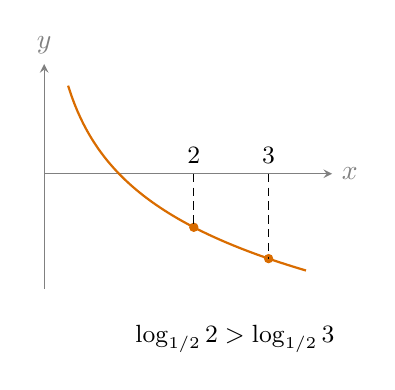
\begin{tikzpicture}[x=0.95cm,y=0.68cm,>=stealth]
 \draw[->,gray] (0,0)--(3.85,0) node[right] {$x$};
 \draw[->,gray] (0,-2.15)--(0,2.05) node[above] {$y$};
 \draw[thick,orange!85!black,domain=0.32:3.5,samples=80] plot (\x,{-ln(\x)/ln(2)});
 \fill[orange!85!black] (2,-1) circle(1.7pt);
 \fill[orange!85!black] (3,{-ln(3)/ln(2)}) circle(1.7pt);
 \draw[densely dashed] (2,0)--(2,-1);
 \draw[densely dashed] (3,0)--(3,{-ln(3)/ln(2)});
 \node[above] at (2,0) {\small $2$};
 \node[above] at (3,0) {\small $3$};
 \node[below] at (2.55,-2.65) {\small $\log_{1/2}2>\log_{1/2}3$};
\end{tikzpicture}
\end{center}
\textbf{读图：}图中取$a=1/2$作代表；较小真数对应更高的点。
\textbf{\textcolor{CExample}{解题步骤：}}
	\begin{description}[style=nextline, leftmargin=2.8em, labelsep=0.5em, itemsep=0.45em]
		\item[\textbf{第一步（分析单调性）：}] 由条件$\log_a 2>\log_a 3$且$2<3$，可知函数$y=\log_a x$在$(0,+\infty)$上为减函数。
			\par\textbf{理由：} 当底数$0<a<1$时，对数函数递减，真数大函数值反而小。
		\item[\textbf{第二步（确定范围）：}] 减函数对应$0<a<1$，结合对数定义域要求$a>0,a\neq1$，得$a\in(0,1)$。
			\par\textbf{理由：} 对数函数分类讨论规则。
	\end{description}

	\textbf{\textcolor{CExample}{关键结论：}}
$0<a<1$。


\textbf{最快判断：}较小的真数$2$反而得到更大的函数值，说明图像必须向右下降，故$0<a<1$。

\medskip

\end{examplebox}
\clearpage
\begin{examplebox}
\textbf{\textcolor{CExample}{例4（高考常见题型：含参数的对数不等式）}}

\textbf{题目：}设$a>0$且$a\ne1$，解不等式
\[
 \log_a(2x-1)>\log_a(x+2).
\]
\textbf{为什么想到：}先保留两个真数都大于0，再看底数决定曲线高低。

\begin{center}\begin{tikzpicture}[font=\small,>=stealth,line join=round]
\draw[gray!40,rounded corners=3pt] (0,0) rectangle (14.2,8.8);\node at (7.1,8.200000000000001) {例4：同一组真数，底数改变会反转两条曲线的高低};
\node at (3.1500000000000004,7.3) {$a=2$};\begin{scope}[shift={(0.4059999999999999,4.65)},x=0.9800000000000001cm,y=0.4125cm]\draw[->,gray] (0.3,0)--(5.3,0) node[right]{$x$};\draw[->,gray] (0,-4)--(0,4) node[above]{$y$};\draw[blue!75!black,thick,solid,domain=0.55:5,samples=180] plot(\x,{ln(2*\x-1)/ln(2)});\draw[violet,thick,dashed,domain=0.55:5,samples=180] plot(\x,{ln(\x+2)/ln(2)});\fill[orange!85!black] (3,2.321928094887362) circle(2pt);\draw[gray!35,densely dotted] (3,0)--(3,-4);\node[below=3pt] at (3,-4){$3$};\draw[gray,densely dotted] (3,0)--(3,2.321928094887362);\end{scope}\node[align=center,text width=5.8cm] at (3.1500000000000004,1.7) {实线：$\log_a(2x-1)$\\虚线：$\log_a(x+2)$};\node at (9.95,7.3) {$a=\frac12$};\begin{scope}[shift={(7.2059999999999995,4.65)},x=0.9800000000000001cm,y=0.4125cm]\draw[->,gray] (0.3,0)--(5.3,0) node[right]{$x$};\draw[->,gray] (0,-4)--(0,4) node[above]{$y$};\draw[orange!85!black,thick,solid,domain=0.55:5,samples=180] plot(\x,{ln(2*\x-1)/ln(0.5)});\draw[teal,thick,dashed,domain=0.55:5,samples=180] plot(\x,{ln(\x+2)/ln(0.5)});\fill[orange!85!black] (3,-2.321928094887362) circle(2pt);\draw[gray!35,densely dotted] (3,0)--(3,-4);\node[below=3pt] at (3,-4){$3$};\draw[gray,densely dotted] (3,0)--(3,-2.321928094887362);\end{scope}\node[align=center,text width=5.8cm] at (9.95,1.7) {实线：$\log_a(2x-1)$\\虚线：$\log_a(x+2)$};
\node[text width=12.6cm,align=center] at (7.1,.65) {两图同尺度，均只画共同定义域x>1/2内；实线高于虚线的区间正是所求。};
\end{tikzpicture}\end{center}

\textbf{第一步：}先保留真数限制：$2x-1>0$且$x+2>0$，合并为$x>\tfrac12$。

\textbf{第二步：}底数分两类。
\begin{itemize}[leftmargin=*,itemsep=0.3em]
 \item 若$a>1$（递增），原式等价于$2x-1>x+2$，即$x>3$，且已满足$x>\tfrac12$。
 \item 若$0<a<1$（递减），原式等价于$2x-1<x+2$，即$x<3$，与定义域合并，得$\tfrac12<x<3$。
\end{itemize}
\textbf{答案：}
\[
\boxed{\begin{cases}
 x>3,&a>1,\\[2pt]
 \tfrac12<x<3,&0<a<1.
\end{cases}}
\]

\begin{center}
\begin{tikzpicture}[x=1cm,y=0.7cm,>=stealth]
 \node[left] at (-0.05,1.18) {\small $a>1$};
 \node[left] at (-0.05,0) {\small $0<a<1$};
 \foreach \yy in {0,1.18}{\draw[->,gray] (0,\yy)--(4.85,\yy);}
 \draw[blue!75!black,very thick,->] (3,1.18)--(4.72,1.18);
 \draw[blue!75!black,fill=white,thick] (3,1.18) circle (2.3pt);
 \draw[orange!85!black,very thick] (0.5,0)--(3,0);
 \draw[orange!85!black,fill=white,thick] (0.5,0) circle(2.3pt);
 \draw[orange!85!black,fill=white,thick] (3,0) circle(2.3pt);
 \node[below] at (0.5,-0.08) {\small $\tfrac12$};
 \node[below] at (3,-0.08) {\small $3$};
 \node[above] at (3,1.24) {\small $3$};
\end{tikzpicture}
\par\small 两个底数区间对应不同解集，空心点表示边界不取。
\end{center}

\textbf{最快判断：}先列“真数大于零”，再按底数分流，最后取交集；\textbf{不能直接去掉对数符号后忘记变号}。

\medskip

\end{examplebox}
\clearpage
\begin{examplebox}
\textbf{\textcolor{CExample}{例5（选择题速判：不同底数不用小数计算）}}

\textbf{题目：}比较$\log_2 3$与$\log_3 2$的大小。

\textbf{为什么想到：}两个底数不同，先试好算的高度1作中间值。

\begin{center}\begin{tikzpicture}[font=\small,>=stealth,line join=round]
\draw[gray!40,rounded corners=3pt] (0,0) rectangle (14.2,8.8);\node at (7.1,8.200000000000001) {例5：用高度1作桥梁，两边分别落在1的上下};
\node at (3.1500000000000004,7.3) {$y=\log_2x$};\begin{scope}[shift={(1.041860465116279,4.466666666666667)},x=1.1395348837209303cm,y=0.7333333333333334cm]\draw[->,gray] (-0.3,0)--(4,0) node[right]{$x$};\draw[->,gray] (0,-2)--(0,2.5) node[above]{$y$};\draw[blue!75!black,thick,solid,domain=0.3:3.8,samples=180] plot(\x,{ln(\x)/ln(2)});\fill[orange!85!black] (2,1) circle(2pt);\fill[orange!85!black] (3,1.5849625007211563) circle(2pt);\draw[gray!35,densely dotted] (2,0)--(2,-2);\node[below=3pt] at (2,-2){$2$};\draw[gray!35,densely dotted] (3,0)--(3,-2);\node[below=3pt] at (3,-2){$3$};\draw[gray,dashed] (.2,1)--(3.8,1);\end{scope}\node[align=center,text width=5.8cm] at (3.1500000000000004,1.7) {$3>2$\\$\log_23>\log_22=1$};\node at (9.95,7.3) {$y=\log_3x$};\begin{scope}[shift={(7.841860465116279,4.466666666666667)},x=1.1395348837209303cm,y=0.7333333333333334cm]\draw[->,gray] (-0.3,0)--(4,0) node[right]{$x$};\draw[->,gray] (0,-2)--(0,2.5) node[above]{$y$};\draw[violet,thick,solid,domain=0.3:3.8,samples=180] plot(\x,{ln(\x)/ln(3)});\fill[orange!85!black] (2,0.6309297535714574) circle(2pt);\fill[orange!85!black] (3,1) circle(2pt);\draw[gray!35,densely dotted] (1,0)--(1,-2);\node[below=3pt] at (1,-2){$1$};\draw[gray!35,densely dotted] (2,0)--(2,-2);\node[below=3pt] at (2,-2){$2$};\draw[gray!35,densely dotted] (3,0)--(3,-2);\node[below=3pt] at (3,-2){$3$};\draw[gray,dashed] (.2,1)--(3.8,1);\end{scope}\node[align=center,text width=5.8cm] at (9.95,1.7) {$1<2<3$\\$0<\log_32<1$};
\node[text width=12.6cm,align=center] at (7.1,.65) {两图同尺度；比较不同底数，分别与好算的1比较，不必求出小数。};
\end{tikzpicture}\end{center}

因为$2^1=2<3$且底数$2>1$，所以$\log_2 3>1$。又因为$3^0=1<2<3^1=3$，所以$0<\log_3 2<1$。因此
\[
 \boxed{\log_3 2<1<\log_2 3}.
\]

\begin{center}
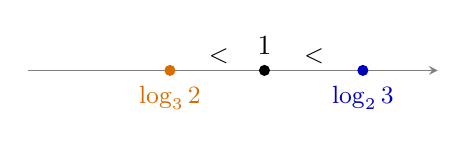
\begin{tikzpicture}[x=1.0cm,y=0.75cm,>=stealth]
 \draw[->,gray] (0,0)--(5.2,0);
 \fill[orange!85!black] (1.8,0) circle(2pt);
 \fill[black] (3,0) circle(2pt);
 \fill[blue!75!black] (4.25,0) circle(2pt);
 \node[below,orange!85!black] at (1.8,-0.1) {\small $\log_3 2$};
 \node[above] at (3,0.1) {$1$};
 \node[below,blue!75!black] at (4.25,-0.1) {\small $\log_2 3$};
 \node at (2.42,0.24) {\small $<$};
 \node at (3.63,0.24) {\small $<$};
\end{tikzpicture}
\par\small 只需要知道两者分别在$1$的左边或右边，不必算小数。此数轴为大小次序示意，不按数值比例。
\end{center}

\textbf{最快判断：}不同底数直接比较困难时，先试$0$、$1$这些好算的中间值；两边恰好分处$1$两侧，一步排出大小。

\medskip

\end{examplebox}
\clearpage
\begin{examplebox}
\textbf{\textcolor{CExample}{举一反三（图像识别）}}
\textbf{题目：}已知对数图像经过$(4,-2)$，判断底数与单调性。
\textbf{为什么想到：}一个已知点能倒推底数；求出候选后还必须检查底数为正。

\begin{center}\begin{tikzpicture}[font=\small,>=stealth,line join=round]
\draw[gray!40,rounded corners=3pt] (0,0) rectangle (14.2,8.3);\node at (7.1,7.700000000000001) {图像识别：点(4,-2)先确定底数，再判断走势};
\begin{scope}[shift={(1.5615384615384615,3.9499999999999997)},x=1.1538461538461537cm,y=0.7666666666666666cm]\draw[->,gray] (-0.4,0)--(4.8,0) node[right]{$x$};\draw[->,gray] (0,-3)--(0,3) node[above]{$y$};\draw[orange!85!black,thick,dashed,domain=0.2:4.5,samples=180] plot(\x,{ln(\x)/ln(0.5)});\fill[orange!85!black] (4,-2) circle(2.2pt);\fill[orange!85!black] (1,0) circle(2.2pt);\draw[gray,densely dotted] (4,0)--(4,-2);\draw[gray!35,densely dotted] (1,0)--(1,-3);\node[below=3pt] at (1,-3){$1$};\draw[gray!35,densely dotted] (4,0)--(4,-3);\node[below=3pt] at (4,-3){$4$};\end{scope}\node[anchor=west,align=left,text width=5.0cm] at (8.4,4.0) {$\log_a4=-2$\\[9pt]$a^{-2}=4$\\[9pt]$a^2=\frac14$\\[9pt]底数为正，$a=\frac12$\\[9pt]递减，并与$\log_2x$上下对称};
\node[text width=12.6cm,align=center] at (7.1,.65) {不能把负的候选底数也保留下来；点(4,-2)确实位于底数1/2的对数曲线上。};
\end{tikzpicture}\end{center}

\textbf{最快解法：}

若$y=\log_a x$经过$(4,-2)$，则$\log_a4=-2\Longleftrightarrow a^{-2}=4$，即$a^2=\tfrac14$。结合\textbf{底数必须为正}，得$a=\tfrac12$。因此它是递减图像，且关于$x$轴翻折后为$y=\log_2x$的图像。
\end{examplebox}
